\documentclass[11pt]{article}
\usepackage[spanish]{babel}

%%%%%%%%%%%%%%%%%%%%%%%%%%%%%%%%%%
%%%%%%%%%%%%%%%%%%%%%%%%%%%%%   %%
%%        Datos Trabajo     %%  %%
%%%%%%%%%%%%%%%%%%%%%%%%%%%%%%%%%%
\newcommand{\titulo}[0]{Actividad 3. Medidas de tendencia central y dispersión.}
\newcommand{\materia}[0]{Estadística Básica}
\newcommand{\grupo}[0]{BI-BEBA-2002-B2-013}
\newcommand{\unidad}[0]{Unidad 3}


%%%%%%%%%%%%%%%%%%%%%%%%%%%%%%%%%%
%%%%%%%%%%%%%%%%%%%%%%%%%%%%%%%%%%
\usepackage{amssymb}
\usepackage{enumerate}
\usepackage{geometry}
\usepackage{mathtools}
\usepackage{multicol}
\usepackage{soul}

\usepackage{graphicx}
	\graphicspath{ {assets/} }

\usepackage{hyperref}
	\hypersetup{
			pdftex,
		        pdfauthor={bench},
		        pdftitle={\titulo},
		        pdfsubject={\materia},
		        pdfkeywords={\grupo, \unidad, UnADM},
		        pdfproducer={Latex with hyperref, Ubuntu},
		        pdfcreator={pdflatex, or other tool},
			colorlinks=true,
				linkcolor=[rgb]{0,0,0.45},
				urlcolor=cyan,
				filecolor=green,
				citecolor=blue}

%%%%%%%%%%%%%%%%%%%%%%%%%%%%%%%%%%
%%%%%%%%%%%%%%%%%%%%%%%%%%%%%%%%%%

\title{
	
\includegraphics{../../../assets/logo-unadm} \\
	\ \\ Benjam\'in Rivera \\
	\bf{\titulo}\\\ \\}

\author{
	Universidad Abierta y a Distancia de México \\
	TSU en Biotecnolog\'ia \\
	\textit{Materia:} \materia \\
	\textit{Grupo:} \grupo \\
	\textit{Unidad:} \unidad \\
	\\
	\textit{Matricula:} ES202105994 }

\date{\textit{Fecha de entrega:} \today}


%%%%%%%%%%%%%%%%%%%%%%%%%%%%%
%%        Documento         %%
%%%%%%%%%%%%%%%%%%%%%%%%%%%%%%%
\begin{document}
\maketitle\newpage

\subsection*{Intruducci\'on}

	\par Continuando con el contenido del curso, y especialmente el de esta unidad en la que estamos aprendiendo a entender los datos; nos encontramos con las medidas de dispersión.
	\par Las \textbf{medidas de dispersión y tendencia central} son valores que nos ayudan a comprender cuales son los datos centrales (con distintas connotaciones) y la manera en que general se comportan los datos respecto al promedio (que es una de las medidas de tendencia central); cada uno respectivamente.
	\par Gracias a estos podemos cálculos podemos obtener ciertas distribuciones e identificar clases que cumplan con ciertas características con más facilidad.
	
	\par \
	\par De manera más específica tratare de poner una breve descripción de las que considero son los cálculos más importantes.
	
	\begin{quote}
		\begin{description}
			\item [El promedio] es el valor del dato que numéricamente se representa centralmente entre todos los demás de la muestra, o población en dicho caso. Puede no estar contenido en los datos de muestra.
			\item [La moda] es el valor que más se repite en los datos estudiados. Este si debe estar contenido en los datos analizados.
			\item [La mediana] es el valor del dato que \textit{geométricamente} se encuentra a la mitad de la muestra, de manera que a ambos lados se encuentre el $50\%$ del resto de los datos. En cas de que se tenga una cantidad par de datos, se saca el promedio de los dos datos \textit{más centrales}.
			
			\par\ 
			\par\noindent Los tres datos anteriores son medidas de tendencia central y los siguientes son de desviación.
			\par\
			\item [La desviación estándar] es el valor que define, en promedio, \textit{que tanto} se separan los datos del valor medio.
			\item [La varianza] es el cuadrado de la desviación estandar.
		\end{description}
	\end{quote}

\newpage
\section*{Ejercicio}

	\par Todos los datos de el ejercicio solicitado fueron ingresados en una hoja de excel y mediante algunas operaciones que ya pude manejar bien en este, implemente los cálculos que se proponen en el libro. Con todo este procedimiento se obtuvieron los datos mostrados en la Figura~\ref{fig: excel}
	
	\begin{figure}[h]
		\centering
		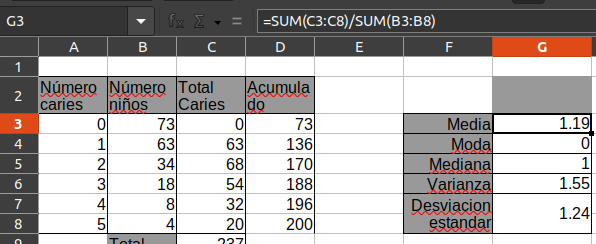
\includegraphics[width=\textwidth]{u3-a3-1.png}
		\caption{Resultados obtenidos en excel.}
		\label{fig: excel}
	\end{figure}
	
	\par De manera que, respecto a los datos del ejercicio propuesto, tenemos que:
	\begin{quote}
		\begin{description}
			\item [El promedio] es $1.19$
			\item [La moda] es $0$
			\item [La mediana] es $1$
			\item [La varianza] es $1.55$
			\item [La desviación estándar] es $1.24$ 
		\end{description}
	\end{quote}
	
	\begin{figure}[htp]
		\centering
		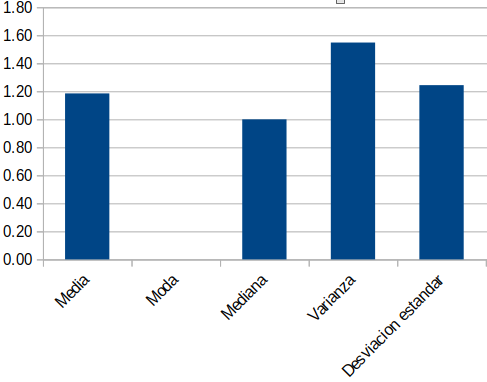
\includegraphics[width=\textwidth]{assets/graficas-A3-U3.png}
		\caption{Gráficas de medidas de tendencia central y dispersión.}
		\label{graficas}
	\end{figure}



%%%%%%%%%%%%%%%%%%%%%%%%%%%%%%%%
%%         Bibliografia        %%
%%%%%%%%%%%%%%%%%%%%%%%%%%%%%%%%%%

\begin{thebibliography}{X}
	\bibitem{basica} Universidad Abierta y a Distancia de México. (s/f). \textit{Unidad 3. Representación numérica y gráfica de datos}. UnADM.
 
\end{thebibliography}

\end{document}